\documentclass[12pt,a4paper]{article}
\usepackage[utf8]{inputenc}
\usepackage[francais]{babel}
\usepackage{enumerate}
\usepackage{ulem}
\usepackage{graphicx}


\begin{document}

\begin{titlepage}
\begin{center}
% Upper part of the page

\textsc{\LARGE UNIVERSITE BORDEAUX 1 }\\[1.5cm]
\textsc{\huge \bfseries Cahier des besoins }\\[1.5cm]
\textsc{\huge \bfseries VPN EveryWhere }\\[1.5cm]
%title


% Author and supervisor


\Large \begin{flushleft}\textbf{Par: }\\
LIU Song\\
AISSOUS Amine\\
HOCINI Mohamed Fouad\\
SI SABER Mohamed Amine\\
\end{flushleft}

\Large 
\begin{flushright}\textbf{Client: }\\
Samuel Thibault\\

\textbf{Chargé de TD: }\\
Henri Derycke\\
\end{flushright}


\vfill
% Bottom of the page
{\large \today}
\end{center}
\end{titlepage}
\tableofcontents 
\newpage



\section{Introduction au projet}
\subsection{Presentation du VPN}

Le rôle d'un VPN (Virtual Private Network) est de fournir aux utilisateurs et administrateurs du système d'information des conditions d'exploitation, d'utilisation et de sécurité à travers un réseau public identiques à celles disponibles sur un réseau privée. Et aussi permet originellement à un utilisateur nomade de se connecter à un réseau d'entreprise depuis l'autre bout du monde: son ordinateur portable a alors l'impression d'être directement branché au réseau d'entreprise, les paquets passant en fait de manière chiffrée via internet.\\
Ces réseaux offrent des avantages majeurs: \\

\begin{itemize}
\item[•] De hautes performances en terme de bande passante.\\
\item[•] La sécurité et la confidentialité des données: permet à l’utilisateur de crypter sa connexion.\\
\item[•] Le VPN permet de contourner la géo-censure sur Internet: La géo-censure est un système de restriction qui bloque l’accès à un contenu en ligne.
\end{itemize}
\subsection{Travail à réaliser}
L'idée est donc de développer un logiciel facilitant la configuration du VPN, en déterminant automatiquement les paramètres réseau à utiliser selon les disponibilités fournies par le réseau auquel on est connecté.\\
Il prendra en entrée un fichier fourni par le fournisseur de serveur VPN, qui décrit notamment l'adresse IP du serveur VPN, éventuellement un certificat pour vérifier que l'on se connecte au bon serveur, l'adresse IP du serveur DNS à utiliser etc. Il demandera éventuellement à l'utilisateur le login et le password s'il n'est pas renseigné dans le fichier .cube.\\

Dans ce projet nous allons réaliser une application qui permet de chercher un port pour se connecter avec le serveur VPN pour que les utilisateurs peuvent utiliser les réseaux publics pour envoyer les données en sécurité. 
\newpage

\section{Description des besoins}

\subsection{Besoins non fonctionnels}
\subsubsection{Besoins comportementaux}


\paragraph{2.1.1.1 Vitesse: }
La bibliothèque doit être capable de faire un scan des ports dans un temps raisonnable en quelques dizaines de seconds, sauf dans le cas de la recherche exhaustive ou cela pourra prendre un peu plus de temps.
\paragraph{2.1.1.2 Facilité d'utilisation: }
Notre application est destiner au large publique la facilité d’utilisation est primordial, chaque utilisateur quel que soit son niveau de connaissance en informatique doit être capable de l’utiliser c’est pour cela qu’on a opter pour une interface simple d’utilisation, où le fait de cliquer simplement sur le bouton Connect lancera le scan des ports et la génération du fichier de configuration .CUBE ainsi éventuellement la connexion automatique au serveur VPN (cela dépendra de l’avancement du projet ) , si la connexion est réussi un voyant vert s’allume sinon dans le cas contraire le voyant sera rouge.\\

L'interface donne la possibilité aux utilisateurs plus expérimenté dans le domaine informatique de faire une configuration manuelle des paramètres de connexion au serveur VPN,et d'ouvrir le fichier .cube de configuration.\\
Elle doit aussi être facile à installer.
 \setlength{\parskip}{1ex}
\paragraph{2.1.1.3 Robustesse: }
S’il y a un échec dans la recherche des ports la bibliothèque doit être capable de relancer le scan, elle temporise pendant 15 seconde puis refait un nouveau scan de ports car il se pourrait que lors du scan précèdent la recherche n’avait pas donné de résultats car il y’avais un problème de connexion dans le réseau.
\paragraph{2.1.1.4 Les difficultés techniques: }
\begin{itemize}
\item[•] \textbf{Réduire le temps d’attente: }
Faire un scan de tous les ports dans le cas où  les ports les plus connus ne permettent pas la connexion au Serveur VPN cela augmentera le temps de réponse la difficulté c’est de trouver un mécanisme qui permet de réduire ce temps d’attente.\\
\item[•] \textbf{Quand es ce arrêter le scan des ports?: }
Vu que l’application est amenée à travailler dans n’importe quel type de réseau il se pourra qu’elle soit lancé dans un réseau dont la connexion internet n’est pas stable, cela pourra fausser le résultat du scan des ports en indiquant qu’aucun port ne permet de se connecter au VPN, La difficulté est de définir si on doit relancer le scan des ports ou dire que ce n’est pas possible de trouver des ports qui parementent la connexion au serveur VPN, nous avons opter de relancer un deuxième scan automatiquement puis on laissera le choix à l’utilisateur s’il veut réessayer ou pas.
\end{itemize}
\begin{itemize}
\item[•] \textbf{Limitation de nombre des connexions ouvertes: }
Lors du scan des ports il ne faut pas essayer de tester tous les ports à la fois car chaque réseau a un nombre maximal de connexion ouvertes en parallèle, par exemple pour le réseau Free le nombre maximal de connexions parallèle autorisé est de 100.
\subsubsection{Besoins organisationnels}

\item[•] \textbf{Processus de développement: }\\
\begin{itemize}
\item L’équipe est constituée de 4 membres, ayant des tâches qui peuvent ou non être faites en binôme.\\
\item Le projet sera réalisé avec le langage Python\\
\item Le scan des ports doit être sous forme bibliothèque python.
\end{itemize}
\end{itemize}

\subsubsection{Besoins externes}

\paragraph{2.1.3.1 Contraintes de Portabilité: }
L’application doit être utilisable sur différents système d’exploitation (Linux, Windows et MAC OS)

\paragraph{2.1.3.2 Contraintes légales:}
L’implémentation de la phase recherche des ports sera sous forme de bibliothèque python afin qu'elle puisse être réutilisable dans d'autres projets, le code doit être bien clair avec des commentaires en anglais ceci afin de facilité sa réutilisation par d’autre personne.\\

Puisque la bibliothèque réalisant le scanne des ports sera réutilisé dans d’autres projets, nous avons choisi de la mettre l’application sous licence LGPL afin de permettre sa modification et sa distribution.\\

\subsection{Besoins fonctionnels}

\begin{flushleft}
Notre projet consiste à mettre en œuvre un Client VPN permettant de scanner les ports ouverts et de générer des fichiers de configuration qui permet de se connecter au serveur VPN, il est organisé par priorité sur 4 phases notons que seul les deux premières étapes du projet sont obligatoires les deux dernière sont optionnelles et elles seront réaliser seulement dans le cas où il nous restera assez de temps pour le faire.\\
Les 4 phases du projet se présentent comme suit:
\end{flushleft}
\paragraph{ La recherche des ports: }c'est la phase la plus importante de notre travail, elle consiste à rechercher les ports qui permettraient de se connecter au serveur VPN, cette recherche se fera sur 3 niveaux, dans un premier temps on va scanner les ports les plus connus si cela ne donne pas de résultats on passe à la deuxième étape qui consiste à faire un scan sur les ports les moins probables mais qui ont déjà servi à se connecter au serveur VPN sinon dans le 3 ème cas on fera une recherche aléatoire sur tous les ports restants.\\

Le scan des ports se fera en utilisant des paquets UDP/TCP, le principe c'est d'envoyer un paquet TCP/UDP au serveur VPN via un port donné, si la machine ayant envoyée le paquet reçoit une réponse du serveur cela voudrait dire que le port utiliser pour envoyer le paquet est ouvert du coup on aura trouvé un port qui permet de se connecter au serveur VPN on arrête le scan des ports et on passe à l'étape suivante qui est la génération du fichier Config.cube.\\
\begin{itemize}
\item[•]\textbf{Recherche des ports Via des paquets UDP: }
Il est à noter qu’on essaye d’abord de faire un Scan des ports en envoyant des paquets UDP Via les ports UDP les plus connu, le temps de réponse des paquets UDP est meilleur que celui des Paquet TCP.\\

\item[•]\textbf{Recherche des ports Via des paquets TCP: }
Si le scan des ports avec les paquets UDP ne donne rien de concret on Scan les ports en envoyant des paquets TCP via les ports TCP les plus connus.\\

\item[•]\textbf{Recherche exhaustive: }
Au cas où les deux premières étapes de scan ne donnent rien  on passe à la recherche exhaustive qui consiste à tester tous les ports restant en utilisant d’abord des paquets UDP puis TCP.\\
\end{itemize}
\paragraph{Production du fichier de configuration: }une fois que la phase détection de port qui permettra de se connecter au serveur VPN est fini, en utilisant le  numéro de port trouvé dans la phase précédente et le fichier de configuration.cube fourni par le Serveur VPN,  on génère le fichier de configuration qui contiendra les informations nécessaire à la connexion au Serveur VPN (Numéro port, login, password, serveur, certificat, nom de domaine)

\paragraph{Lancement avec le serveur "optionnel": }(OPENVPN par exemple) consiste à lancer la connexion du client au serveur via des lignes de commandes.

\paragraph{ Test "optionnel": } 
Afin de tester  l’application on essaye de se connecter via un port TCP donné à  une adresse IP qui n'est accessible que Via le serveur VPN, si cela marche ça voudrai dire que notre application fonctionne et que ça passe bien par le VPN.

\subsubsection{Graphe des besoins fonctionnels}
\begin{center}
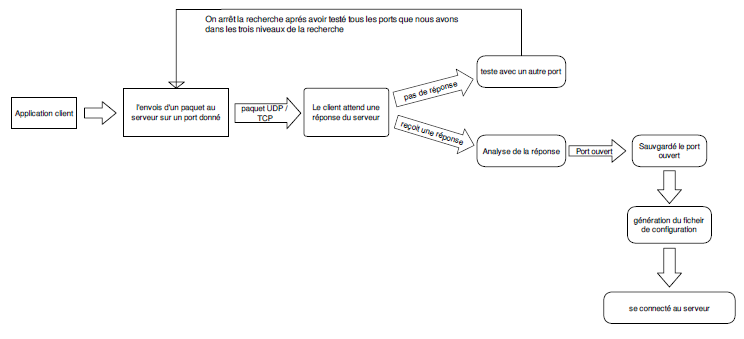
\includegraphics
[width=10cm]{Graphedesbesoinsfonctionnels.PNG}
\end{center}
\begin{center}
{2.2.1: Graphe des besoins fonctionnels }
\end{center}
\subsection{GUI et Graphe de Fonctionnement de l'application}
\textbf
Notre application va permettre à un client de se connecter facilement à un serveur VPN, on a décidé après plusieurs rencontres avec le client de faire une interface simple et pratique. \\
\newpage
\textbf{2.3-1.Fenêtre principale: }\\
\begin{center}
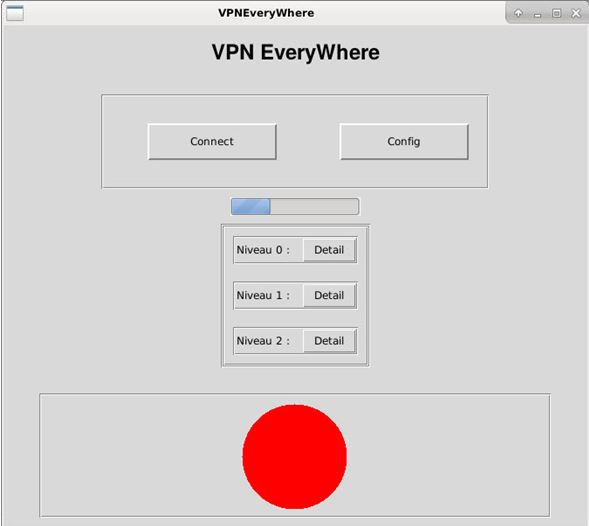
\includegraphics
[width=11cm]{VPNEveryWhere.jpg}
\end{center}
\begin{center}

{2.3-1: Fenêtre principale }
\end{center}


\begin{itemize}
\item Bouton Connecte: permet de lancer le processus de connexion au server VPN passant par les étapes de scan de port \\
\item Bouton Config: permet de configurer les login, password et le choix du serveur.\\
\item Bouton Open configFile: permet d'ouvrir le fichier de configuration .Cube du sevrer .\\
\item Barre de progression: pour afficher l’avancement de la  recherche  par nombres des ports testés et niveau de recherche.\\

\item[•]Bouton Detail: Pour afficher les détails du niveau 1.\\

\item[•]Bouton Detail: Pour afficher les détails du niveau 2.\\

\item[•]Bouton Detail: Pour afficher les détails du niveau 3.\\

\end{itemize}
\newpage
Voyant: on a trois état avec trois couleurs différentes
\begin{itemize}
\item Rouge  : déconnecté du serveur.
\vspace{8pt}
\item Orange : connexion en cours.
\vspace{8pt}
\item Vert   : connecté au serveur.\\
\end{itemize}
\textbf{Message d'erreur: }pour afficher les différents messages d'erreurs que l'utilisateur peut avoir\\

\textbf{2.3-2.Fenêtre Config: \\}
\begin{center}
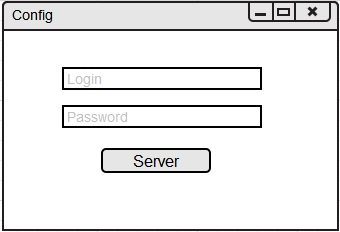
\includegraphics
[width=10cm]{Config.jpg}
\end{center}
\begin{center}
{2.3-2: Fenêtre Config}
\end{center}

\begin{itemize}
\item[•] Login: contient le nom d'utilisateur.\\
\item[•] Password: pour le password de l'utilisateur.\\
\item[•] Server: pour configurer le serveur.\\
\end{itemize}
\newpage
\textbf{2.3-3.Fenêtre Server: \\}

\begin{center}
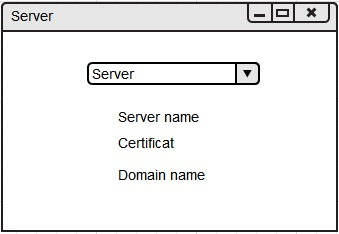
\includegraphics
[width=10cm]{Server.jpg}
\end{center}
\begin{center}
{2.3-3: Fenêtre Server}
\end{center}

Liste déroulante qui contient la liste des serveurs déjà préconfiguré, avec la possibilité de configurer le serveur manuellement.\\
\newpage
\textbf{2.3-4: Graphe de Fonctionnement \\}\\
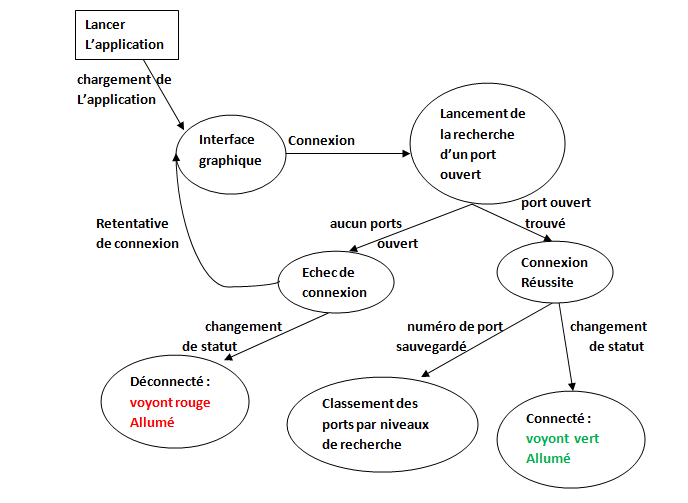
\includegraphics
[width=11cm]{Graphedefonctionement.png}\begin{center}
{2.3-4: Graphe de Fonctionnement}
\end{center}

\subsection{Type d'erreurs}


\begin{enumerate}
\item \textbf{Échec de connexion: }\\
Si on trouve pas de port ouvert.\\
\item \textbf{Échec de login: }\\
Si login ou password ne sont pas correct.\\
\item \textbf{Échec de certificats: }\\
Si le certificats d'utilisateur est invalide ou périmé.\\
\end{enumerate}

\end{document}